\chapter{Implementation}
\section{Data Gathering}
\subsection{Training Dataset}
\subsubsection{TED Talks}
\begin{figure}
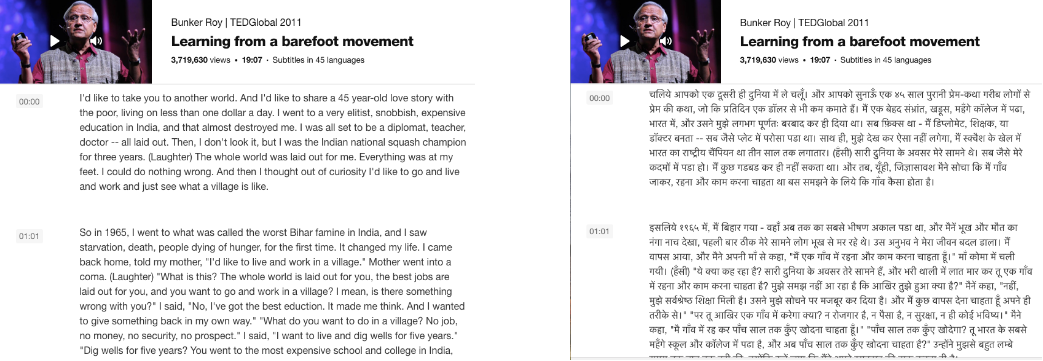
\includegraphics[width=\textwidth]{figures/tedtalks.png}
\caption{A side-by-side figure showing TED Talk transcripts in English and Hindi} \label{fig1}
\end{figure}
\subsubsection{Beautiful Soup}
Beautiful Soup is one of the most widely used open source Python library designed by Leonard Richardson for quick turnaround projects like website scrapping. The decision to use Beautiful Soup for this research was motivated by the fact that It provides simple methods and Pythonic idioms for navigating, searching and modifying a parse tree. It’s a simple toolkit for dissecting the document and extracting the relevant information according to the user’s need. Beautiful Soup makes the handling of encodings much easier, it automatically converts incoming documents to Unicode and outgoing documents to UTF-8. The library sits on top of Popular parsers like lxml and html5lib which allows the user to try different parsing strategies or trade speed for flexibility. 
\subsubsection{Indic NLP Library}
Indic NLP Library is an open source Python Based Library for common text processing and Natural Language Processing in Indian Languages developed by Anoop Kunchukuttan.  The Indian Languages are originated from Sanskrit and are quite different from the Latin-Based Languages or other Asian Languages, so the other NLP Libraries doesn’t perform well on Indian Languages. Though the Indian languages share a lot of similarity among themselves in terms of script, phonology, language syntax, etc. There are very few researches going in the field of Hindi NLP, and Indic NLP Library is the only existing NLP library for the Hindi language. The library provides several functionalities such as Text Normalization, Tokenization, and Morphological Analysis.
\subsubsection{Moses Tokenizer}
Moses is one of the most successful implementations of the Statistical Machine Translation which was the dominant approach before the onset of Neural Machine Translation. Moses provides several tools for Statistical Machine Translation process, such as for Corpus preparation it provides tokenization, true casing and cleaning tools. As the process of preparation of corpus remains same for Neural Machine Translation Systems, the Moses Tokenizer was chosen here for the tokenization of the English text. 
\subsubsection{TED Hindi English Corpus}
\begin{figure}
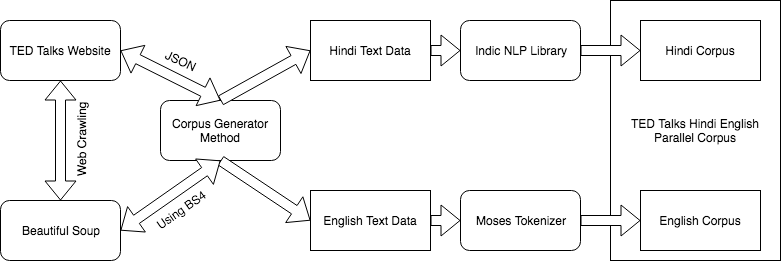
\includegraphics[width=\textwidth]{figures/traindataworkflow.png}
\caption{Workflow of the TED Talks Corpus Generator} \label{fig1}
\end{figure}
TED.com discontinued their Open API project and so there is no direct way to fetch the transcripts of talks. TED.com is a static website, so talks link location is static and can be accessed if prior information of talks details is obtained through Beautiful soup and $urllib$ library in python 

Firstly, the Beautiful Soup library is used to fetch the links of all the 396 TED Talks which are available in the Hindi language from the home page of the TED Official Website. The URL of the web page is passed to the method which implements the Beautiful Soup.  For each and every web page, the $find/_$all() method finds all the “$a$” tags in the respective pages. Further, $attrs$ method is used to find all the $“href”$ which are having "$/talks$". The URL to the original talks is obtained and stored in a list for further parsing. The method is iterated through the entire list of pages having Hindi TED Talks. 

The transcripts for the talks are fetched from TED’s internal server which is having an open access and URL is appended "$transcript.json?language=en$" . Two different methods for English and Hindi are implemented to obtain the JSON from the respective URLs and load into the data file. 

The JSON is parsed by the respective methods and the transcript text is obtained. The JSON data consisted of time frames, translated text of available language which here Hindi and English respectively. The methods parse the JSON data, fetch the translation and write it in two separate text files “$Hindi.txt$” and “$English.txt$” to create the Hindi-English Parallel Corpus.

The text files generated by the methods were ill-formatted and contained junk texts. So, there was a need for Normalization and Tokenization of the text files. The text written in Hindi displays a lot of quirky behavior on varying input or multiple representations of the same character, so there was a need to canonicalize the representation of the text such that the NLP applications can handle the data inconsistent manner. The canonicalization of the text files handled issues such as,
\begin{itemize}
\item Non-Spacing characters like ZWJ/ZWNL
\item Multiple Representations of Nukta based Characters
\item Multiple Representations of two-part dependent vowel signs
\item Typing inconsistencies: e.g. use of pipe ($|$) for poorna virama 
\end{itemize}

Further the tokenizer in the library was used to tokenize the Hindi text and make it ready for corpora.

The Moses tokenizer comes with two perl scripts which takes two

\subsection{Test Data}
\subsubsection{Blog Content from Tripoto}
\subsubsection{Sumy}
Sumy is an Open Source python library and python command line utility for extracting a summary from HTML pages or plain texts, developed by Miso Belica. The package also contains a simple evaluation framework for text summaries.The decision to use sumy was driven by a number of factors.Sumy is an extractive text summarizer.Extractive text summarization techniques perform summarization by extracting portions of texts and constructing a summary, while the abstractive techniques like Google's TextSum learn the internal language representation to generate more human-like summaries,
and paraphrases the original text. Extractive text summarization makes more sense in the summarization of Blogs as it keeps the original text which highlights the author’s point of view and writing style. Secondly, the abstractive text summarization is technique is highly unfeasible considering the available infrastructure at this stage of research.Further, Sumy provides seven different summarization methods which gives a choice to choose the best summarization algorithm for the blog summarization. 

The methods are as follows: 

\begin{itemize}
    \item Luhn is one of the earliest suggested algorithms by the famous IBM researcher it was named after and it scores sentences based on the frequency of the most important words. The algorithm derives statistical information from word frequency and distribution to compute a relative measure of significance. The sentence which scores relatively higher than others is extracted to create a summary. 
    \item Edmundson is a heuristic method which implements previous statistic research of high-frequency words along with the three additional components: pragmatic words (cue words); title and heading words; and structural indicators (sentence location). 
    
\end{itemize}

\subsubsection{Summarizer}

\begin{figure}
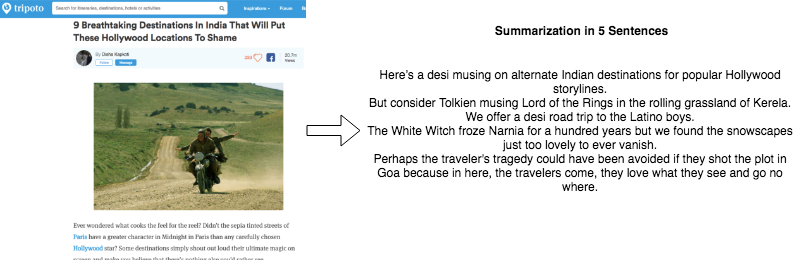
\includegraphics[width=\textwidth]{figures/textsummary.png}
\caption{Histogram of side-by-side scores on 500 sampled sentences from Wikipedia and news websites for a
typical language pair, here English to Spanish (PBMT blue, GNMT red, Human orange). It can be seen that
there is a wide distribution in scores, even for the human translation when rated by other humans, which
shows how ambiguous the task is. It is clear that GNMT is much more accurate than PBMT.} \label{fig1}
\end{figure}
Tripoto is one of the biggest Travel Blogging Websites in the World. The method implements the Beautiful Soup library and fetches the list of 50 most popular blogs from the URL “$https://www.tripoto.com/trips$ “. The links to the respective blogs is written into a csv (comma separated values) file for the summarization.

The method which implements the sumy library reads the csv file and creates a 5-sentence summary for each and every blog. After experimenting with LexRank, TextRank and Latent Semantic Analysis (LSA), LSA is finally used as the summarizer based on the quality of the summary. The Summary is then saved in a csv file corresponding to their blog links, which is further used by the Visual Interface. 

\section{Neural Translation Model}
\subsection{Keras}
Keras is an open source high-level neural networks API, which is written in Python and capable of running on top of TensorFlow, CNTK, and Theano.  It was designed to enable fast experimentation with deep neural networks and make neural network programming more user-friendly, modular and extensible. The decision to use Keras was driven by a number of factors. Firstly, Keras allows for easy and fast prototyping with minimal lines of code, it’s easier to code than TensorFlow.  In Keras, a model is represented as a sequence or a graph of standalone, fully-configurable modules that can be linked together with very limited restrictions. The neural layers, cost functions, optimizers, activation functions, regularization schemes are all standalone modules that can be combined easily to create new models. 
\subsection{Seq2Seq Model}
\section{Visual Interface}
